\documentclass[conference]{IEEEtran}
\usepackage{graphicx,booktabs,amsmath,amssymb,url,xcolor,multirow}
\usepackage[hidelinks]{hyperref}
\newcommand{\todo}[1]{\textcolor{red}{[TODO: #1]}}
\newcommand{\repo}{\url{https://github.com/bob0612/small-lrm-overthinking}}

\begin{document}
\title{Thinking Past the Answer at Small Scale:\\Correct-then-Wrong Reasoning and Label-Free Stopping in 0.6B--4B Reasoning Models}
\author{\IEEEauthorblockN{\todo{Full name}}\IEEEauthorblockA{Student ID 3036797441\\The University of Hong Kong}}
\maketitle

\begin{abstract}
Reasoning models often keep thinking after they already hold the right answer, and sometimes talk themselves out of it.
Recent work measures this ``harmful overthinking'' and the room for early stopping on models of 4B parameters and up,
using the gold answer to decide where an ideal stop would be. We ask two questions at the small end of the scale, where
such models are actually deployed on cheap hardware: how often do Qwen3-0.6B, 1.7B and 4B in thinking mode reach a
correct answer and then abandon it, and how much of the gap to an oracle stopping point can a rule recover that uses no
gold answer and no training? We force an answer every $\sim$128 thinking tokens on GSM8K, MATH-500 and AIME
2024/25 \todo{N} traces, and evaluate fixed budgets, answer-consistency and answer-confidence rules with thresholds
chosen by grouped cross-validation. \todo{key numbers}. Code, data and all traces: \repo.
\end{abstract}

\section{Introduction}
\label{sec:intro}
Thinking-mode language models solve harder problems by writing long chains of thought before answering. The cost is
length: on easy problems they spend thousands of tokens after the answer is already settled
\cite{chen2024overthinking,sui2025stop}. Worse, extra thinking is not always neutral. Caldarella et al.\ show that
stopping at the first correct prefix would raise Qwen3's AIME2025 accuracy from 58.3\% to 91.7\%
\cite{caldarella2026thinking}, and Guan et al.\ find that full thinking is 9.03 points less accurate than the earliest
accuracy peak along the trajectory, averaged over six models \cite{guan2026pareto}. Both papers leave open the practical
question: a stopping policy that does not know the gold answer.

These studies, and most early-exit methods \cite{liu2025convergence,zhang2025know,scalena2026commitment}, use models
of 4B--70B parameters. Small reasoning models (under 2B) are the ones most often run on laptops and phones, where every
token is paid for in latency. Their behaviour may differ: they are weaker, so fewer traces ever reach a correct
answer, and they are known to loop. Whether overthinking at small scale is mostly \emph{wasted} or mostly
\emph{harmful} is an empirical question we could not find answered.

\textbf{Research questions.}
\begin{itemize}
\item[\textbf{RQ1}] How often do 0.6B--4B reasoning models reach a correct intermediate answer and end with a wrong one,
and how does this depend on model size and problem difficulty?
\item[\textbf{RQ2}] How close do simple, training-free stopping rules (fixed budget, answer consistency, answer
confidence) get to an oracle that stops at the first correct answer, when their thresholds are chosen without test
labels?
\item[\textbf{RQ3}] Is the thinking after the answer stabilises still causally used? We change a number in the trace
before and after that point and measure whether the final answer follows.
\end{itemize}

\textbf{Contributions.} \todo{after results}

\section{Related Work}
\label{sec:related}
\textbf{Overthinking and efficient reasoning.} Surveys organise efficient-reasoning methods into model-, output- and
prompt-based approaches \cite{sui2025stop}. Budget forcing caps or extends thinking by editing the trace
\cite{muennighoff2025s1}. Guan et al.\ build offline Pareto frontiers of termination methods for six models and show
that dynamic early exit needs only 14.2\% of the budget to match full-thinking accuracy, while public online methods
stay below their frontiers \cite{guan2026pareto}. Caldarella et al.\ separate verbose from harmful overthinking and note
that practical policies without ground truth remain open \cite{caldarella2026thinking}.

\textbf{Signals for stopping.} Liu and Wang stop when intermediate answers converge and cut 40\% of tokens on NQ, but
report that convergence is not correctness on GPQA and AIME \cite{liu2025convergence}. Hidden-state probes predict
correctness with ROC-AUC above 0.7 and enable 24\% savings at equal accuracy \cite{zhang2025know}; a probe on Qwen3-8B
predicts the final outcome from the first few tokens \cite{david2025temporal}. These probes need training data and
access to activations; our rules need neither.

\textbf{Faithfulness of reasoning.} Interventions on chains of thought test whether the answer depends on them
\cite{lanham2023faithfulness}. Scalena et al.\ find a commitment boundary after which corrupting numbers leaves the
answer unchanged in 95\% of runs, in 14B--26B models with greedy decoding \cite{scalena2026commitment}. Monitorability
of reasoning is now treated as a safety property \cite{korbak2025monitorability}. We repeat the corruption test at
0.6B--4B with sampling and a clean-resampling control.

\section{Method}
\label{sec:method}
\subsection{Answer trajectories}
For a problem $x$ we sample one thinking trace $z = (z_1,\dots,z_L)$ ending at the \texttt{</think>} token (or at the
cap of 8{,}192 tokens). We choose probe points $t_1<\dots<t_m=L$ roughly every 128 tokens, moved back to the nearest
line end so that a probe never splits a sentence. At each $t_j$ we feed
$x \,\|\, z_{1:t_j} \,\|$ \texttt{</think>}\,\texttt{The final answer is \$\textbackslash boxed\{} and decode greedily
until the box closes. This gives an answer $a_j$, its probability $c_j=\prod p(\text{answer tokens})$, and the number of
hesitation words (``wait'', ``hmm'', \dots) so far. With prefix caching \cite{vllm} each probe only costs the new
tokens. The sequence $(a_j, c_j)_{j=1}^m$ is the \emph{answer trajectory}. At the model's own stopping point we use the
answer it actually writes after \texttt{</think>} as $a_m$, not the forced probe: forcing a box immediately after
\texttt{</think>} occasionally drops a sign or a square root that the model's own answer keeps, and we report this
probe noise separately (Section~\ref{sec:limits}).

\subsection{Outcome categories}
Let $y_j=\mathbb{1}[a_j \text{ is correct}]$. A trace is \emph{never} correct if all $y_j=0$; \emph{kept} if $y_m=1$ and
some earlier $y_j=1$; \emph{late} if only $y_m=1$; and \emph{flip} (correct-then-wrong, harmful overthinking) if some
$y_j=1$ but $y_m=0$. The \emph{oracle stop} answers at the first correct probe, which upper-bounds any stopping rule
that only chooses among probed answers.

\subsection{Stopping rules}
A rule sees $(a_i,c_i,t_i)_{i\le j}$ and decides whether to stop at $t_j$, answering $a_j$:
\begin{itemize}
\item \textbf{Fixed budget} $B$: stop at the first $t_j\ge B$.
\item \textbf{Consistency} $(k, t_{\min})$: stop when the last $k$ answers agree and $t_j\ge t_{\min}$.
\item \textbf{Confidence} $\tau$: stop when $c_j\ge\tau$.
\item \textbf{Consistency + confidence} $(k,\tau)$: both.
\end{itemize}
A rule that never fires answers $a_m$. Cost is the number of thinking tokens used.

\subsection{Selecting thresholds without test labels}
We split problems into five folds, grouping both samples of a problem in the same fold. On four folds we pick the rule
with the fewest tokens whose accuracy is within 0.5 points of full thinking on those folds, and report its accuracy and
tokens on the held-out fold. This is the deployment question: \emph{if I tune a stopping rule on some labelled problems,
what do I save on new ones?}

\subsection{Commitment test}
For a sample of traces in each category we cut the thinking at 25/50/75/90\% of its length, change the last number in
the cut (e.g.\ $x\to x\pm d$ or $2x$), and sample a continuation. A clean continuation from the same cut is the control,
since sampling alone changes answers. The causal dependence at a position is the difference between how often the
final answer changes under corruption and under clean resampling.

\section{Experimental Setup}
\label{sec:setup}
\textbf{Models.} Qwen3-0.6B, 1.7B and 4B \cite{qwen3} in thinking mode, bf16, sampling with the recommended
temperature 0.6, top-$p$ 0.95, top-$k$ 20; two samples per problem. \textbf{Data.} 500 problems sampled from the GSM8K test
set \cite{gsm8k} (seed 0), MATH-500 \cite{math,lightman2024verify} and the 60 AIME 2024/2025 problems. Answers are
compared after normalisation and with \texttt{math-verify}. \textbf{Compute.} One NVIDIA A40 (48\,GB) rented for
\todo{h} hours (\todo{\$}), vLLM 0.11.0. \todo{exact model commits from config.json}.

\section{Results}
\label{sec:results}
Each model produced 2{,}120 traces (1{,}060 problems $\times$ 2 samples). Table~\ref{tab:outcomes} gives accuracy,
the oracle and the outcome categories; Fig.~\ref{fig:traj} shows how the forced answer improves along the trace.

\begin{table}[t]
\centering
\caption{Accuracy of full thinking (the model's own answer), accuracy of the oracle that stops at the first correct
probe, share of correct-then-wrong (flip) and never-correct traces, and mean thinking tokens. All numbers in \%, except
tokens.}
\label{tab:outcomes}
\scriptsize
\setlength{\tabcolsep}{3.5pt}
\begin{tabular}{llrrrrrr}
\toprule
Model & Data & Acc. & Oracle & Flip & Never & Tokens & Oracle tok. \\
\midrule
0.6B & GSM8K & 78.8 & 83.1 & 4.3 & 16.9 & 1681 & 927 \\
 & MATH-500 & 71.6 & 79.1 & 7.5 & 20.9 & 3794 & 2313 \\
 & AIME & 10.8 & 13.3 & 2.5 & 86.7 & 7539 & 7226 \\
 & All & 71.6 & 77.3 & 5.7 & 22.7 & 3009 & 1937 \\
\midrule
1.7B & GSM8K & 91.5 & 94.4 & 2.9 & 5.6 & 1911 & 685 \\
 & MATH-500 & 88.3 & 90.7 & 2.4 & 9.3 & 3920 & 1649 \\
 & AIME & 28.3 & 30.0 & 1.7 & 70.0 & 7763 & 6623 \\
 & All & 86.4 & 89.0 & 2.6 & 11.0 & 3190 & 1476 \\
\midrule
4B & GSM8K & 94.7 & 96.6 & 1.9 & 3.4 & 1930 & 530 \\
 & MATH-500 & 94.1 & 95.4 & 1.3 & 4.6 & 3818 & 1282 \\
 & AIME & 51.7 & 55.0 & 3.3 & 45.0 & 7535 & 5698 \\
 & All & 92.0 & 93.7 & 1.7 & 6.3 & 3138 & 1178 \\
\bottomrule
\end{tabular}

\end{table}

\begin{figure}[t]
\centering
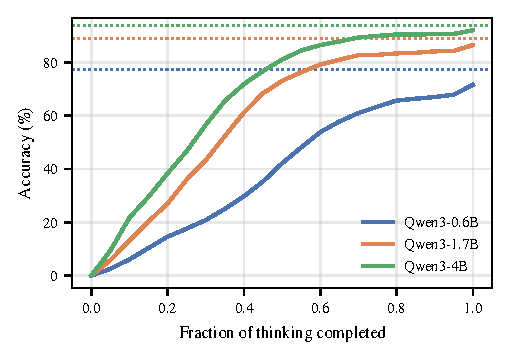
\includegraphics[width=0.85\columnwidth]{figures/trajectory.pdf}
\caption{Accuracy of the forced answer against the fraction of the trace completed (all datasets). Dotted lines:
oracle stop. Larger models reach most of their final accuracy in the first half of the trace.}
\label{fig:traj}
\end{figure}

\subsection{RQ1: harmful overthinking is rare and shrinks with scale; wasted thinking grows}
Correct-then-wrong traces exist at every size but are a small minority: 5.7\% of all traces for 0.6B (95\% CI
4.7--6.8), 2.6\% for 1.7B (1.9--3.4) and 1.7\% for 4B (1.1--2.4). As a share of traces that were ever correct this is
7.4\%, 2.9\% and 1.8\%. The flip rate thus falls by a factor of three from 0.6B to 4B, while accuracy rises from 71.6\%
to 92.0\%. Stopping at the first correct probe would add 5.7, 2.6 and 1.7 points (Table~\ref{tab:outcomes}); these
gains are smaller than the 9--33 points reported for larger models on AIME \cite{guan2026pareto,caldarella2026thinking},
largely because most of our problems are easier and a weak model's errors are mostly \emph{never} correct (22.7\% of
0.6B traces) rather than flips.

The waste is a different story. On traces that are ever correct, 57\%, 70\% and 75\% of the thinking comes after the
first correct probe, and the oracle would use 36\%, 54\% and 63\% fewer tokens. Larger models reach the answer earlier
(Fig.~\ref{fig:traj}: at half the trace 4B's forced answer is already 81\% accurate, 0.6B's only 42\%) but do not stop
earlier: all three spend about 3{,}000--3{,}200 tokens on average. Overthinking at this scale is therefore mostly
\emph{wasted}, and increasingly so with size, while \emph{harmful} overthinking is concentrated in the smallest model.

Within MATH-500, the 0.6B flip rate is highest on level-5 problems (11.6\% against 4.8--6.7\% for levels 1--4;
Fig.~\ref{fig:level}); for 1.7B and 4B the rate stays at or below 3.5\% at every level. On GSM8K, which is easy for all
three models, flips still occur in 4.3\%, 2.9\% and 1.9\% of traces. AIME traces are mostly truncated at our 8{,}192-token
cap (79\% for 1.7B), so we do not interpret the AIME rows.

\begin{figure}[t]
\centering
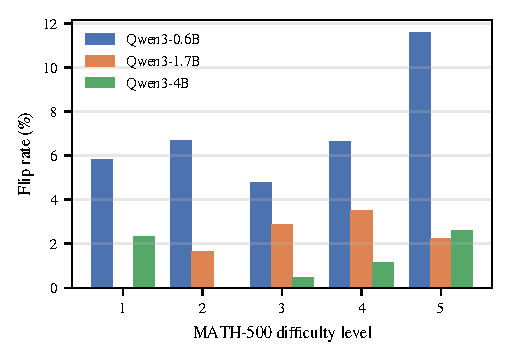
\includegraphics[width=0.85\columnwidth]{figures/flip_by_level.pdf}
\caption{Flip rate by MATH-500 difficulty level.}
\label{fig:level}
\end{figure}

\textbf{What predicts a flip?} Table~\ref{tab:pred} compares signals available at the first correct probe, without the
gold answer, between flip and kept traces. The strongest is the probability the model assigns to its forced answer:
flips start from a less confident correct answer (mean 0.45 vs 0.72 for 0.6B), giving an AUC of 0.75 for 0.6B when
read in that direction, falling to 0.58 for 4B. Flips also find the correct answer \emph{earlier} in the trace (AUC
0.71 for 0.6B, reversed), so a lucky early guess is more fragile than a derived one. Hesitation words separate the
classes only for 4B (AUC 0.64), and the number of distinct earlier answers is uninformative at all sizes.

\begin{table}[t]
\centering
\caption{Separating flip from kept traces at their first correct probe: AUC of each signal (0.5 = chance; values
below 0.5 mean low values predict a flip).}
\label{tab:pred}
\scriptsize
\begin{tabular}{lrrr}
\toprule
Signal at first correct probe & 0.6B & 1.7B & 4B \\
\midrule
Answer confidence & 0.75\,$\downarrow$ & 0.64\,$\downarrow$ & 0.58\,$\downarrow$ \\
Distinct answers so far & 0.55 & 0.56 & 0.52\,$\downarrow$ \\
Relative position & 0.71\,$\downarrow$ & 0.64\,$\downarrow$ & 0.63\,$\downarrow$ \\
Hesitations / 1k tok. & 0.55\,$\downarrow$ & 0.57 & 0.64 \\
Difficulty level & 0.62 & 0.51 & 0.53 \\
\midrule
\# flip traces & 121 & 55 & 36 \\
\bottomrule
\end{tabular}

\end{table}

\subsection{RQ2: label-free rules recover little of the oracle's savings}
Fig.~\ref{fig:pareto} plots each rule family's accuracy--token frontier against full thinking and the oracle, and
Table~\ref{tab:cv} gives the held-out result of tuning thresholds by grouped cross-validation. The oracle sits far above
every frontier: it is both more accurate than full thinking and 36--63\% cheaper. No rule matches full thinking
accuracy within 0.5 points at any meaningful saving: even in-sample, every rule that saves tokens loses more than half a
point on the pooled data, and under cross-validation the selected rule saves 2.1\%, 0.0\% and 4.7\% of tokens. Allowing a
2-point loss, cross-validation selects a 4{,}096-token budget for 0.6B (27.5\% saved, $-1.7$ points) and
consistency-plus-confidence rules for 1.7B and 4B (11.7\% and 21.8\% saved, $-1.6$ and $-1.8$ points).

The rules do better on easy data. On GSM8K alone, the 0.5-point setting saves 17\%, 14\% and 23\% of tokens, and the
2-point setting 28\%, 31\% and 47\%. On MATH-500 the 0.5-point setting saves nothing for 1.7B and 4B. Answer
confidence alone is the weakest family: its frontier lies well below the others for every model, because a
small model is often confidently wrong early in the trace. Consistency rules fail in a related way: the early answers
of a hard problem can agree with each other and still be wrong, which is exactly the failure mode reported for larger
models on AIME and GPQA \cite{liu2025convergence}.

\begin{figure*}[t]
\centering
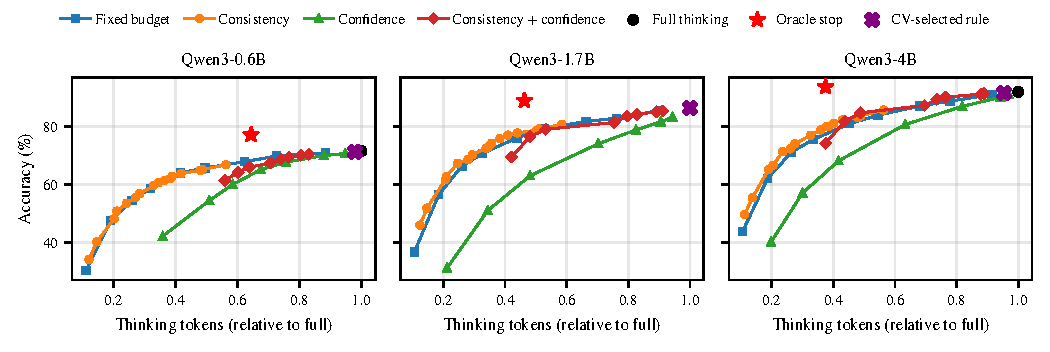
\includegraphics[width=0.9\textwidth]{figures/pareto.pdf}
\caption{Accuracy against mean thinking tokens (relative to full thinking) for the Pareto frontier of each rule
family, pooled over datasets. Black: full thinking. Red star: oracle stop at the first correct probe. Purple: the
rule chosen by grouped 5-fold cross-validation (held-out).}
\label{fig:pareto}
\end{figure*}

\begin{table}[t]
\centering
\caption{Held-out effect of the cross-validated rule, at two accuracy tolerances used for selection. ``Saved'' is
the share of thinking tokens saved relative to full thinking.}
\label{tab:cv}
\scriptsize
\setlength{\tabcolsep}{3pt}
\begin{tabular}{lrrrrrr}
\toprule
 & \multicolumn{2}{c}{Full thinking} & \multicolumn{2}{c}{Oracle stop} & \multicolumn{2}{c}{CV rule (acc. / saved)} \\
Model & Acc. & Tok. & Acc. & Saved & $\le$0.5\,pp & $\le$2\,pp \\
\midrule
0.6B & 71.6 & 3009 & 77.3 & 35.6\% & 71.3 / 2.1\% & 69.9 / 27.5\% \\
1.7B & 86.4 & 3190 & 89.0 & 53.7\% & 86.4 / 0.0\% & 84.8 / 11.7\% \\
4B & 92.0 & 3138 & 93.7 & 62.5\% & 91.6 / 4.7\% & 90.2 / 21.8\% \\
\bottomrule
\end{tabular}

\end{table}

\subsection{RQ3: the thinking after the answer settles is still used}
\todo{commitment results}

\section{Discussion and Limitations}
\label{sec:limits}
\todo{discussion after all results}

\textbf{Probes are a reading, not the model's answer.} A forced answer is what the model writes when made to stop,
which is the right quantity for a stopping rule but can differ from what it would write after a natural stop. At the
end of thinking, where both exist, they disagree on 4.2\%, 1.1\% and 0.5\% of traces for 0.6B, 1.7B and 4B (8.4\% on MATH-500 for 0.6B), mostly in format: a dropped sign or square root, or a different number from the forced reading. We
therefore count harmful overthinking only when an intermediate probe is correct, and use the model's own answer at the
end; residual probe noise can still create spurious ``correct'' intermediate probes, so our flip rates are upper bounds
on genuine answer reversals.

\textbf{Scope.} One model family, one sampling setting, two samples per problem, mathematics only, and a probe every
$\sim$128 tokens (finer probing would only move the oracle earlier). AIME results rest on 60 problems and are mostly
truncated at 8{,}192 tokens, so we report them but do not draw conclusions from them. Thresholds are tuned per model;
we did not test transfer across models or datasets. The commitment test changes one number; other corruptions
(deleting a step, inserting a wrong claim) may give different dependence.

\section{Conclusion}
\todo{}

\section*{Reproducibility and AI Use}
All code, the exact commands, per-trace outputs and the analysis are in \repo. AI coding assistance (Claude, Anthropic)
was used for code and drafting; all numbers come from the scripts in the repository.

\bibliographystyle{IEEEtran}
\bibliography{references}
\end{document}
